% Standalone vector figure extracted from manuscript.tex.
% Rebuild all figures from the project root: bash tkz/build.sh
\documentclass[tikz,border=2pt,class=IEEEtran]{standalone}
\usepackage{amsmath,amssymb,amsfonts}
\usepackage{xcolor}
\usetikzlibrary{positioning,arrows.meta,calc,backgrounds}

% Match the manuscript's IEEE Access text and math font settings.
\renewcommand{\textbf}[1]{{\fontseries{b}\selectfont #1}}
\renewcommand{\textit}[1]{{\itshape #1}}
\makeatletter
\AtBeginDocument{%
  \fontencoding{T1}\rmfamily\fontseries{m}\fontsize{10}{12}\selectfont
  \gdef\operator@encoding{T1}%
  \gdef\encodingdefault{T1}}
\makeatother

% ---- shared palette for review figures ----
\definecolor{cVLA}{HTML}{34618E}   % VLA lane / policy blue
\definecolor{cWM}{HTML}{9E4A3F}    % world-model lane
\definecolor{cCONV}{HTML}{5E4B8B}  % convergence purple
\definecolor{cGood}{HTML}{3A7D44}  % verified green
\definecolor{cWarn}{HTML}{B07A2A}  % caution amber
\definecolor{cPale}{HTML}{F2F0EA}  % pale panel fill
\tikzset{
  fnode/.style={draw=black!55, fill=white, rounded corners=1.5pt,
                inner sep=2.5pt, align=center, font=\fontsize{8}{9.5}\selectfont},
  flane/.style={draw=none, rounded corners=2pt, inner sep=3pt,
                align=center, font=\fontsize{8}{9.5}\selectfont\bfseries, text=white},
  farr/.style={-{Stealth[length=2mm]}, thick, black!60},
}


\newcommand{\figfont}{\fontsize{8}{9.5}\selectfont}

\begin{document}

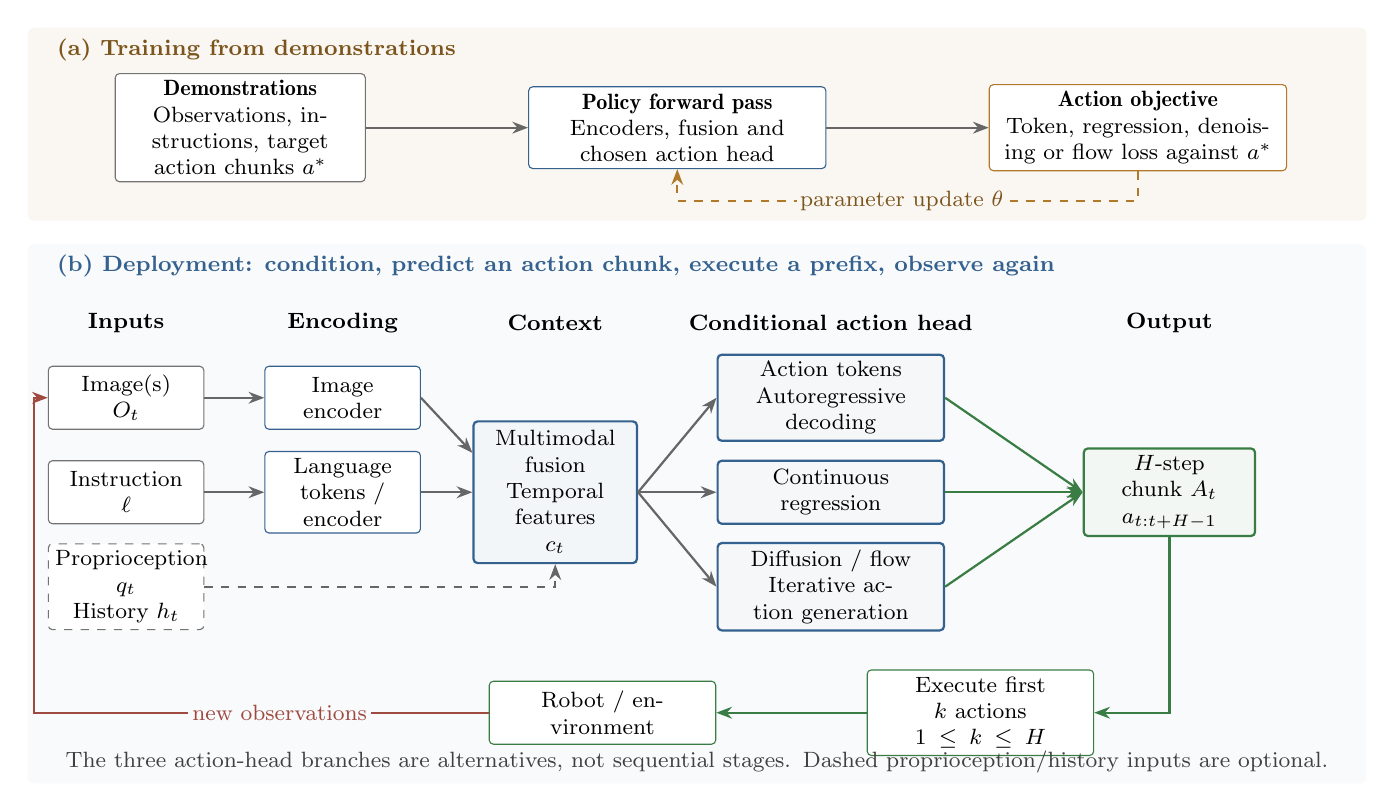
\begin{tikzpicture}[font=\figfont]
\tikzset{box/.style={fnode,minimum height=8mm},
 head/.style={box,draw=cVLA,thick,fill=cVLA!5,text width=27mm},
 title/.style={font=\fontsize{8.5}{10}\selectfont\bfseries,anchor=west}}
% Training is visually separate from the deployed sensor/action loop.
\fill[cWarn!6,rounded corners=2pt] (0,.6) rectangle (17,3.05);
\node[title,text=cWarn!70!black] at (.25,2.77) {(a) Training from demonstrations};
\node[box,text width=30mm] (data) at (2.7,1.78) {\textbf{Demonstrations}\\Observations, instructions, target action chunks $a^*$};
\node[box,draw=cVLA,text width=36mm] (train) at (8.25,1.78) {\textbf{Policy forward pass}\\Encoders, fusion and chosen action head};
\node[box,draw=cWarn,text width=36mm] (loss) at (14.1,1.78) {\textbf{Action objective}\\Token, regression, denoising or flow loss against $a^*$};
\draw[farr] (data)--(train);\draw[farr] (train)--(loss);
\draw[farr,dashed,cWarn] (loss.south)--(14.1,.85)--(8.25,.85)--(train.south);
\node[fill=cWarn!6,inner sep=1pt,text=cWarn!70!black] at (11.1,.85) {parameter update $\theta$};
% Main deployment pipeline: alternative heads branch in parallel.
\fill[cVLA!3,rounded corners=2pt] (0,-6.55) rectangle (17,.3);
\node[title,text=cVLA] at (.25,.02) {(b) Deployment: condition, predict an action chunk, execute a prefix, observe again};
\node[font=\figfont\bfseries] at (1.25,-.7) {Inputs};
\node[font=\figfont\bfseries] at (4,-.7) {Encoding};
\node[font=\figfont\bfseries] at (6.7,-.7) {Context};
\node[font=\figfont\bfseries,align=center] at (10.2,-.7) {Conditional action head};
\node[font=\figfont\bfseries] at (14.5,-.7) {Output};
\node[box,fill=white,text width=18mm] (images) at (1.25,-1.65) {Image(s)\\$O_t$};
\node[box,fill=white,text width=18mm] (language) at (1.25,-2.85) {Instruction\\$\ell$};
\node[box,dashed,text width=18mm] (extra) at (1.25,-4.05) {Proprioception $q_t$\\History $h_t$};
\node[box,draw=cVLA,text width=18mm] (vision) at (4,-1.65) {Image encoder};
\node[box,draw=cVLA,text width=18mm] (text) at (4,-2.85) {Language tokens / encoder};
\node[box,draw=cVLA,thick,fill=cVLA!6,text width=19mm,minimum height=18mm] (fusion) at (6.7,-2.85) {Multimodal fusion\\Temporal features\\$c_t$};
\draw[farr] (images)--(vision);\draw[farr] (language)--(text);
\draw[farr] (vision.east)--([yshift=5mm]fusion.west);
\draw[farr] (text.east)--(fusion.west);
\draw[farr,dashed] (extra.east)--(6.7,-4.05)--(fusion.south);
\node[head] (tokens) at (10.2,-1.65) {Action tokens\\Autoregressive decoding};
\node[head] (regression) at (10.2,-2.85) {Continuous regression};
\node[head] (diffusion) at (10.2,-4.05) {Diffusion / flow\\Iterative action generation};
\foreach \headnode in {tokens,regression,diffusion}{\draw[farr] (fusion.east)--(\headnode.west);}
\node[box,draw=cGood,thick,fill=cGood!6,text width=20mm] (chunk) at (14.5,-2.85) {$H$-step chunk $A_t$\\$a_{t:t+H-1}$};
\foreach \headnode in {tokens,regression,diffusion}{\draw[farr,cGood] (\headnode.east)--(chunk.west);}
\node[box,draw=cGood,text width=27mm] (execute) at (12.1,-5.65) {Execute first $k$ actions\\$1\le k\le H$};
\node[box,draw=cGood,text width=27mm] (robot) at (7.3,-5.65) {Robot / environment};
\draw[farr,cGood] (chunk.south)--(14.5,-5.65)--(execute.east);
\draw[farr,cGood] (execute)--(robot);
\draw[farr,cWM] (robot.west)--(.08,-5.65)--(.08,-1.65)--(images.west);
\node[text=cWM,fill=cVLA!3,inner sep=1.5pt] at (3.2,-5.65) {new observations};
\node[align=center,text width=163mm,text=black!75] at (8.5,-6.27)
 {The three action-head branches are alternatives, not sequential stages. Dashed proprioception/history inputs are optional.};
\end{tikzpicture}
\end{document}
